\documentclass[14pt]{extarticle}

\begin{document}
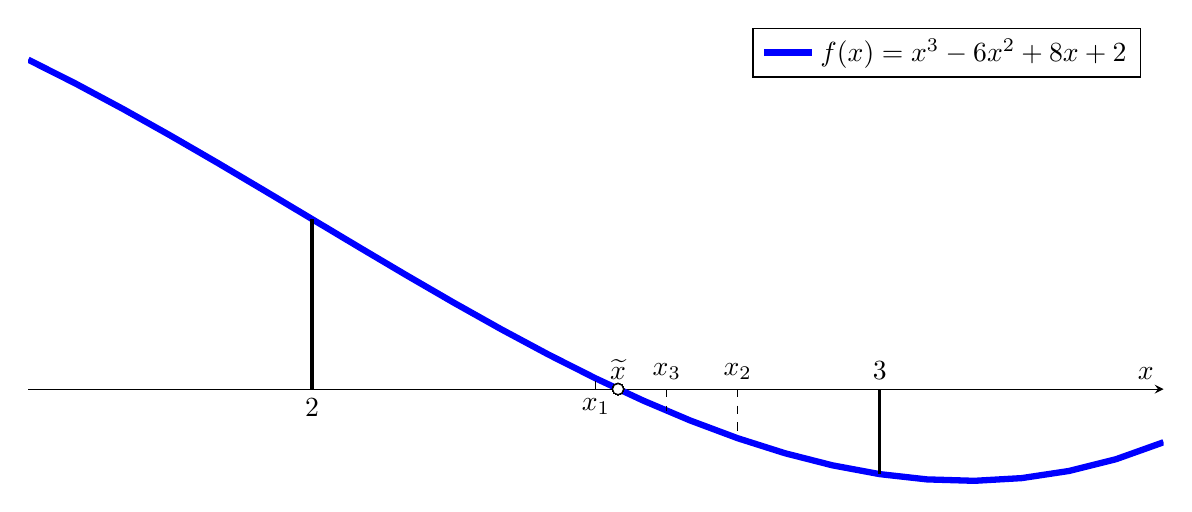
\begin{tikzpicture} [
	declare function={
		f(\x)= \x^3 - 6*\x^2+ 8*\x + 2;
	},
]
	\begin{axis} [
		height=8cm,
		width=16cm,
		xlabel = {$x$},
		ylabel = {$f(x)$},
		axis x line = middle,
		hide y axis,
		domain = 1.5:3.5,
		ticks = none ]

		\newcommand*{\varA}{2}
		\newcommand*{\varB}{3}
		\newcommand*{\X}{2.539}
		\pgfmathsetmacro{\fb}{f(\varB)}
		\pgfmathsetmacro{\fa}{f(\varA)}
		\pgfmathsetmacro{\Xfirst}{(\varA+\varB)/2}
		\pgfmathsetmacro{\fXfirst}{f(\Xfirst)}
		\pgfmathsetmacro{\Xsecond}{(\Xfirst+\varB)/2}
		\pgfmathsetmacro{\fXsecond}{f(\Xsecond)}
		\pgfmathsetmacro{\Xthird}{(\Xfirst+\Xsecond)/2}
		\pgfmathsetmacro{\fXthird}{f(\Xthird)}

		\addplot[color=blue, line width=.08cm]{f(x)};

		\coordinate(A) at 	(\varA,		\fa);
		\node[below](Ap) at 	(\varA,		0) {$\varA$};
		\coordinate(B) at 	(\varB,		\fb);
		\node[above](Bp) at 	(\varB,		0) {$\varB$};
		\node[above](X) at 	(\X,		0)
			{$\widetilde{x}$};
		\coordinate(X1) at 	(\Xfirst,	\fXfirst);
		\node[below](X1p) at 	(\Xfirst,	0) {$x_1$};
		\coordinate(X2) at 	(\Xsecond,	\fXsecond);
		\node[above](X2p) at 	(\Xsecond,	0) {$x_2$};
		\coordinate(X3) at 	(\Xthird,	\fXthird);
		\node[above](X3p) at 	(\Xthird,	0) {$x_3$};

		\addplot[mark=*,only marks, fill=white] (\X, 0)
			node[above, pos=1]{};

		\draw[very thick] (Ap) -- (A)	(Bp) -- (B);
		\draw[dashed] (X1p) -- (X1)	(X2p) -- (X2)
			(X3p) -- (X3);

		\addlegendentry{$f(x)=x^3-6x^2+8x+2$};
	\end{axis}
\end{tikzpicture}
\end{document}
